\section{Introduction}
\label{sec:intro}

Vision-language models (VLMs) such as CLIP~\cite{radford2021clip} and SigLIP~\cite{zhai2023siglip} classify an image by comparing its embedding with text embeddings of class names. The zero-shot classifier is general but frozen: it ignores the structure of the data it is applied to. A growing family of methods therefore adapts it from the unlabeled test data itself, transductively on a batch~\cite{martin2024transductive,zanella2024transclip,kalantidis2024zlap,li2025ecalp} or online on a stream~\cite{karmanov2024tda,zhang2024dmn,zhang2024dpe,fuchs2025oga}, training nothing and operating on cached features.

Two recent studies temper the enthusiasm. Zanella \etal~\cite{zanella2025stata} show that when a batch contains only a few of the vocabulary classes, which is the common case for a photo album, a surveillance feed or a user session, transductive methods lose tens of accuracy points with respect to the zero-shot model they are meant to improve, and Sheng \etal~\cite{sheng2025illusion} report that test-time adaptation methods deliver marginal gains, transfer poorly to backbones other than CLIP and degrade calibration. The remedy proposed in~\cite{zanella2025stata}, and refined in~\cite{huang2026moon}, is a statistical anchor: each class prototype is shrunk towards its text embedding with a strength that depends on how many test samples the class receives. Anchoring prevents collapse, but it treats every class as an island. A class that receives no samples stays exactly at its text anchor, although the anchor is known to be displaced from the image distribution by the modality gap and by the domain of the test data~\cite{liang2022gap,schrodi2025two}; a class with one or two samples is adapted from those samples alone.

\begin{figure}[t]
  \centering
  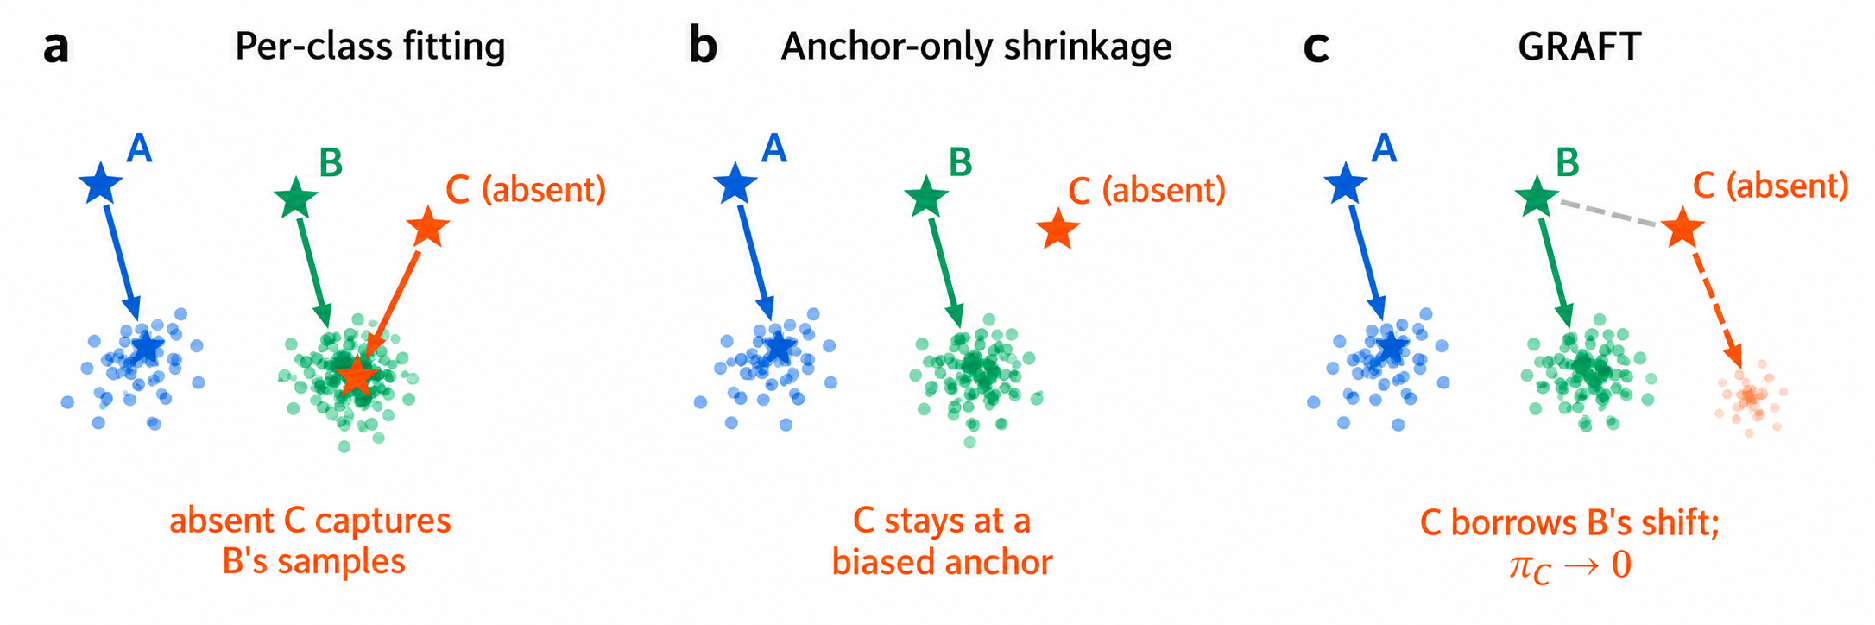
\includegraphics[width=\linewidth]{figures/fig3_concept.pdf}
  \caption{\textbf{Per-class adaptation on a realistic batch (conceptual).} Classes A and B are present, C is absent, and all images are shifted from their anchors. (a) Per-class fitting lets C capture samples of B. (b) Anchor-only shrinkage leaves C at its biased anchor. (c) \method lets C inherit B's displacement and removes it through the presence model.}
  \label{fig:concept}
\end{figure}

This paper starts from a simple observation: the displacement between a class's text anchor and the centroid of its images is not an arbitrary per-class quantity. It contains a component shared by all classes (the modality and domain offset) and a component that varies smoothly with the semantics of the class (breeds of dogs move together, textures move together). We turn this observation into a prior. \method models the adapted prototypes as $\mu_k = t_k + d_k$ and places a Gaussian Markov random field prior on the displacement field $D = [d_1;\dots;d_K]$ whose precision is $\alpha I + \lambda L_T$, where $L_T$ is the Laplacian of a $k$-nearest-neighbour graph over the text embeddings. The $\alpha$ term reproduces the anchor-only shrinkage of~\cite{zanella2025stata,huang2026moon}; the $\lambda$ term is new and couples the classes, so that the displacement of a class with many samples propagates to its semantic neighbours. The maximum a posteriori field has a closed form, $D = (N_z + s(\alpha I + \lambda L_T))^{-1} N_z E$, where $N_z$ holds the soft counts and $E$ the empirical displacements: a graph filter that returns the empirical displacement for well-observed classes and the harmonic extension of the neighbours' displacements for absent ones (\cref{fig:concept}c). Classes that receive no samples are additionally removed from the competition by a Dirichlet-regularised estimate of the class proportions, which treats the vocabulary as a label-shift problem~\cite{saerens2002adjusting,garg2020unified} rather than as a fixed set of equally likely competitors.

\method is training free and gradient free: all updates are closed form on cached features, the online variant keeps a few sufficient statistics per class, and the prior strengths can be chosen by maximising the marginal likelihood of the unlabeled batch, removing the hyper-parameters that the critique of~\cite{sheng2025illusion} targets. Our contributions are:
\begin{enumerate}
  \item a formulation of transductive VLM adaptation in which the class prototypes form a displacement field with a graph-structured prior over the class vocabulary, together with the closed-form block-coordinate inference that fits it on batches and streams (\cref{sec:method});
  \item an analysis showing that anchor-only shrinkage and a single global shift are the two extreme settings of the proposed prior, that absent classes receive the harmonic extension of present-class displacements through the Kron-reduced class graph, and that the posterior variance of every prototype is never larger than under independent shrinkage (\cref{sec:analysis});
  \item an explicit class-presence model and an empirical Bayes rule for the prior strength, which remove the dataset-specific tuning of the pooling strength;
  \item an implementation with unit-tested closed-form updates that plugs into the realistic batch and online protocols of~\cite{zanella2025stata}, with a pre-registered experimental plan (\cref{sec:experiments}).
\end{enumerate}
